% Work done by a force along a path from point 1 to point 2
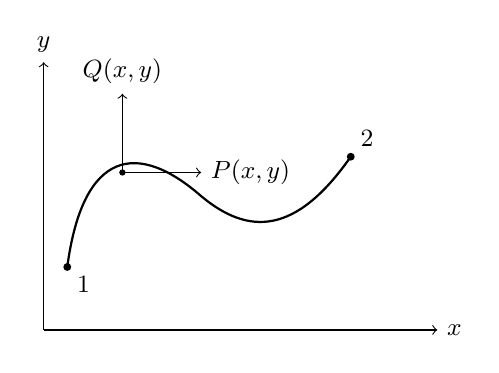
\begin{tikzpicture}[scale=1.0,font=\small]
  \draw[->] (0,0) -- (5.0,0) node[right] {$x$};
  \draw[->] (0,0) -- (0,3.4) node[above] {$y$};
  \draw[thick] (0.3,0.8) .. controls (0.5,2.3) and (1.2,2.4) .. (2.0,1.7)
               .. controls (2.6,1.2) and (3.2,1.2) .. (3.9,2.2);
  \fill (0.3,0.8) circle (0.05) node[below right] {1};
  \fill (3.9,2.2) circle (0.05) node[above right] {2};
  \coordinate (Q) at (1.0,2.0);
  \fill (Q) circle (0.04);
  \draw[->] (Q) -- ++(1.0,0) node[right] {$P(x,y)$};
  \draw[->] (Q) -- ++(0,1.0) node[above] {$Q(x,y)$};
\end{tikzpicture}
